% UIR-2 report (English version), variant 51/51/30. Compile with XeLaTeX:  xelatex report_en.tex (twice)
\documentclass[12pt,a4paper]{article}
\usepackage{fontspec}
\IfFontExistsTF{Times New Roman}{\setmainfont{Times New Roman}}{\setmainfont{Liberation Serif}}
\IfFontExistsTF{Courier New}{\setmonofont{Courier New}[Scale=0.9]}{\setmonofont{Liberation Mono}[Scale=0.9]}
\usepackage[english]{babel}
\usepackage[left=25mm,right=15mm,top=20mm,bottom=20mm]{geometry}
\usepackage{amsmath,amssymb}
\usepackage{graphicx,float,caption,subcaption}
\usepackage{booktabs,multirow,array,longtable,multicol}
\usepackage{tikz}
\usetikzlibrary{arrows.meta,positioning,fit}
\usepackage{indentfirst}
\usepackage{listings,xcolor}
\usepackage[hidelinks]{hyperref}
\captionsetup{labelsep=endash}
\setlength{\parskip}{3pt}
\linespread{1.1}
\emergencystretch=3em
\lstset{basicstyle=\ttfamily\footnotesize, breaklines=true, frame=single, columns=fullflexible,
        showstringspaces=false, keywordstyle=\color{blue!60!black}, commentstyle=\color{gray}, language=Python}

\makeatletter\newcommand{\tabinput}[1]{\@@input #1 }\makeatother
\newcommand{\SoneThr}{0.1890}
\newcommand{\StwoThr}{0.1000}
\newcommand{\Ratio}{1.89}
\newcommand{\SonePi}{0.6220}
\newcommand{\StwoPi}{0.8000}
\newcommand{\SoneU}{25.06}
\newcommand{\StwoU}{37.88}
\newcommand{\SoneL}{2.846}
\newcommand{\StwoL}{2.788}
\newcommand{\SoneRho}{0.9451}
\newcommand{\StwoRho}{0.99996}
\newcommand{\SoneR}{1.8901}
\newcommand{\SoneThrA}{0.0980}
\newcommand{\SoneThrB}{0.0910}
\newcommand{\SonePiA}{0.6986}
\newcommand{\SonePiB}{0.4797}
\newcommand{\StwoExpThr}{0.0999}
\newcommand{\StwoExpU}{37.56}
\newcommand{\SoneSymThr}{0.1921}
\newcommand{\SoneZero}{0.001822}
\newcommand{\StwoZero}{0.000036}
\newcommand{\SoneFull}{0.335118}
\newcommand{\StwoFullSum}{0.8000}
\newcommand{\SoneMaxRes}{4.2\cdot10^{-17}}
\newcommand{\StwoMaxRes}{7.4\cdot10^{-17}}
% ---------- transition graph of SYSTEM_1 ----------
\newcommand{\graphOne}{%
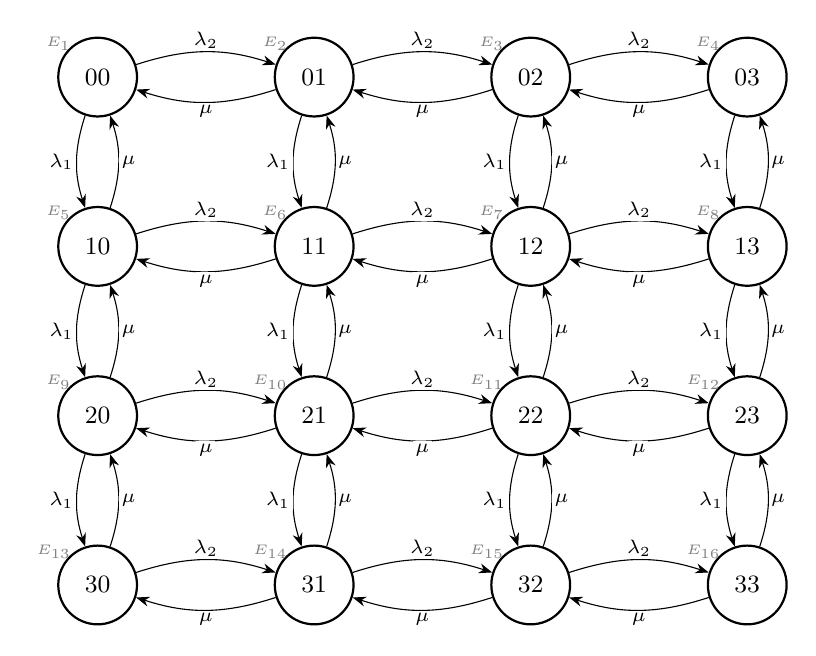
\begin{tikzpicture}[>=Stealth, st/.style={circle, draw, thick, minimum size=10mm, inner sep=0pt, font=\small},
  lab/.style={font=\scriptsize, fill=white, inner sep=1pt}, x=2.75cm, y=2.15cm]
\foreach \a in {0,...,3}{\foreach \c in {0,...,3}{
  \pgfmathtruncatemacro{\k}{\a*4+\c+1}
  \node[st] (s\a\c) at (\c,-\a) {\a\c};
  \node[font=\tiny, text=gray, above left=-1.5mm and -1.5mm of s\a\c] {$E_{\k}$};
}}
\foreach \a in {0,...,3}{\foreach \c [evaluate=\c as \cn using int(\c+1)] in {0,1,2}{
  \draw[->] (s\a\c) to[bend left=18] node[lab, above]{$\lambda_2$} (s\a\cn);
  \draw[->] (s\a\cn) to[bend left=18] node[lab, below]{$\mu$} (s\a\c);
}}
\foreach \c in {0,...,3}{\foreach \a [evaluate=\a as \an using int(\a+1)] in {0,1,2}{
  \draw[->] (s\a\c) to[bend right=18] node[lab, left]{$\lambda_1$} (s\an\c);
  \draw[->] (s\an\c) to[bend right=18] node[lab, right]{$\mu$} (s\a\c);
}}
\end{tikzpicture}}

% ---------- transition graph of SYSTEM_2 ----------
\newcommand{\graphTwo}{%
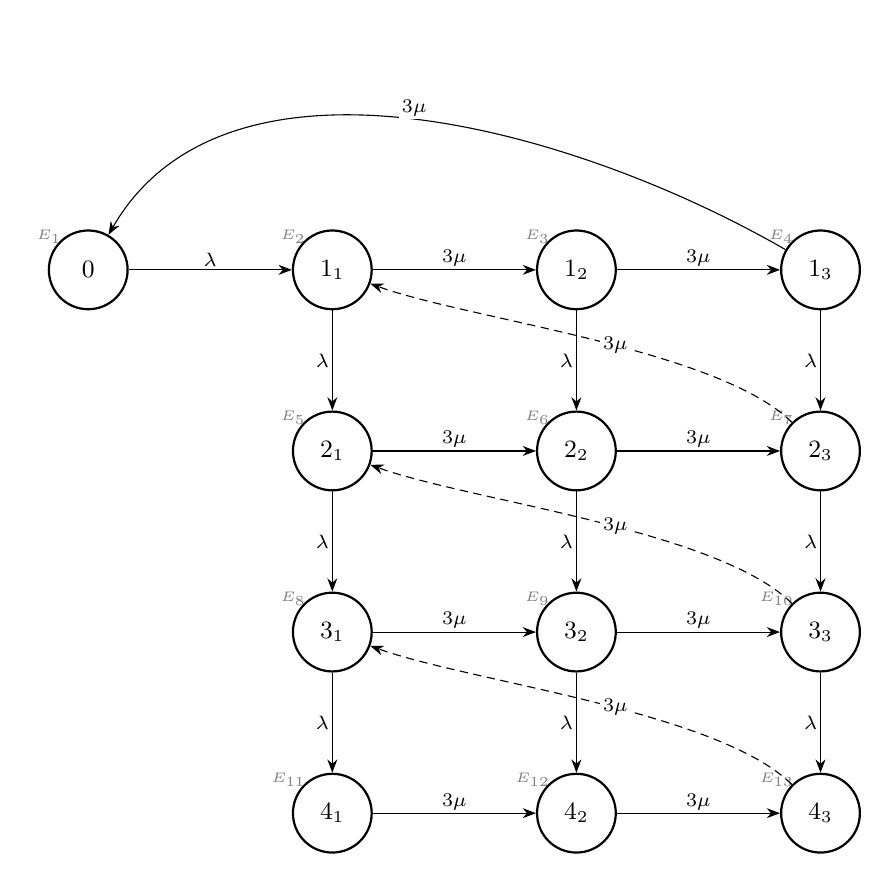
\begin{tikzpicture}[>=Stealth, st/.style={circle, draw, thick, minimum size=10mm, inner sep=0pt, font=\small},
  lab/.style={font=\scriptsize, fill=white, inner sep=1pt}, x=3.1cm, y=2.3cm]
\node[st] (s0) at (0,-1) {$0$};
\node[font=\tiny, text=gray, above left=-1.5mm and -1.5mm of s0] {$E_{1}$};
\foreach \n in {1,...,4}{\foreach \j in {1,2,3}{
  \pgfmathtruncatemacro{\k}{(\n-1)*3+\j+1}
  \node[st] (s\n\j) at (\j,-\n) {$\n_{\j}$};
  \node[font=\tiny, text=gray, above left=-1.5mm and -1.5mm of s\n\j] {$E_{\k}$};
}}
% phase transitions
\foreach \n in {1,...,4}{
  \draw[->] (s\n1) -- node[lab, above]{$3\mu$} (s\n2);
  \draw[->] (s\n2) -- node[lab, above]{$3\mu$} (s\n3);
}
% arrivals
\draw[->] (s0) -- node[lab, above]{$\lambda$} (s11);
\foreach \j in {1,2,3}{\foreach \n [evaluate=\n as \nn using int(\n+1)] in {1,2,3}{
  \draw[->] (s\n\j) -- node[lab, left]{$\lambda$} (s\nn\j);
}}
% departures (end of phase 3)
\draw[->] (s13) to[out=150, in=60, looseness=0.9] node[lab, above]{$3\mu$} (s0);
\foreach \n [evaluate=\n as \np using int(\n-1)] in {2,3,4}{
  \draw[->, densely dashed] (s\n3) to[out=135, in=-20, looseness=0.6] node[lab, pos=0.45]{$3\mu$} (s\np1);
}
\end{tikzpicture}}

% ---------- structural schemes ----------
\newcommand{\schemeOne}{%
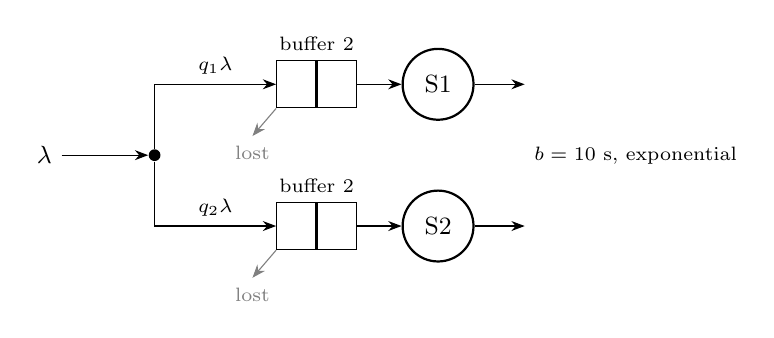
\begin{tikzpicture}[>=Stealth, font=\small,
  srv/.style={circle, draw, thick, minimum size=9mm}, buf/.style={rectangle, draw, minimum width=5mm, minimum height=6mm}]
\node (src) at (0,0) {$\lambda$};
\node[circle, fill, inner sep=1.5pt] (sp) at (1.4,0) {};
\draw[->] (src) -- (sp);
\foreach \y/\i/\q in {0.9/1/q_1, -0.9/2/q_2}{
  \node[buf] (b\i a) at (3.2,\y) {}; \node[buf, right=0pt of b\i a] (b\i b) {};
  \node[srv] (p\i) at (5.0,\y) {S\i};
  \draw[->] (sp) |- node[pos=0.75, above, font=\scriptsize]{$\q\lambda$} (b\i a.west);
  \draw[->] (b\i b) -- (p\i); \draw[->] (p\i) -- ++(1.1,0) node[right]{};
  \node[above=0pt of b\i a.north east, font=\scriptsize] {buffer 2};
  \draw[->, gray] (b\i a.south west) ++(0,0) -- ++(-0.3,-0.35) node[below, font=\scriptsize]{lost};
}
\node[right, font=\scriptsize] at (6.1,0) {$b=10$ s, exponential};
\end{tikzpicture}}

\newcommand{\schemeTwo}{%
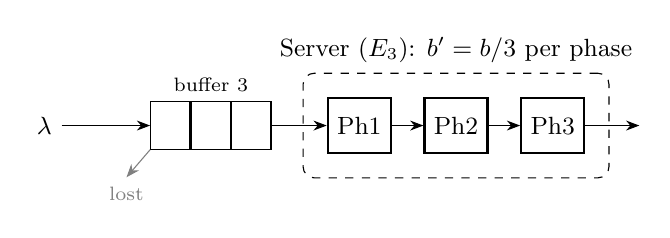
\begin{tikzpicture}[>=Stealth, font=\small,
  ph/.style={rectangle, draw, thick, minimum width=8mm, minimum height=7mm}, buf/.style={rectangle, draw, minimum width=5mm, minimum height=6mm}]
\node (src) at (0,0) {$\lambda$};
\node[buf] (b1) at (1.6,0) {}; \node[buf, right=0pt of b1] (b2) {}; \node[buf, right=0pt of b2] (b3) {};
\node[above=0pt of b2.north, font=\scriptsize] {buffer 3};
\node[ph] (f1) at (4.0,0) {Ph1}; \node[ph, right=4mm of f1] (f2) {Ph2}; \node[ph, right=4mm of f2] (f3) {Ph3};
\node[draw, dashed, rounded corners, fit=(f1)(f3), inner sep=3mm, label={above:{Server ($E_3$): $b'=b/3$ per phase}}] {};
\draw[->] (src) -- (b1); \draw[->] (b3) -- (f1); \draw[->] (f1) -- (f2); \draw[->] (f2) -- (f3); \draw[->] (f3) -- ++(1.1,0);
\draw[->, gray] (b1.south west) -- ++(-0.3,-0.35) node[below, font=\scriptsize]{lost};
\end{tikzpicture}}


\begin{document}
% ======================= TITLE =======================
\begin{titlepage}
\centering
{\large ITMO University\\Faculty of Software Engineering and Computer Systems\par}
\vspace{5cm}
{\Large Course: Modeling\par}
\vspace{1cm}
{\LARGE\bfseries Research Assignment No.\,2 (UIR-2)\par}
\vspace{0.4cm}
{\Large ``Markov Models of Queueing Systems''\par}
\vspace{0.6cm}
{\large Variant 51/51/30\par}
\vfill
\begin{flushright}
\begin{tabular}{l}
Student: Rahaman Md Afifur, group P3330\\[4mm]
Instructor: \rule{4.5cm}{0.4pt}\\
\end{tabular}
\end{flushright}
\vspace{2cm}
Saint Petersburg, 2026
\end{titlepage}

\tableofcontents
\newpage

% ======================= 1 =======================
\section{Objective and problem statement}
\textbf{Objective:} to study the method of Markov random processes and apply it to queueing
systems with a homogeneous flow of requests.

\textbf{Task:} build Markov models of two alternative queueing systems (SYSTEM\_1 and SYSTEM\_2),
compute the stationary state probabilities and the performance characteristics, compare the systems
and choose the better one according to the given efficiency criterion.

\subsection{Input data}
Assignment variant: $N1/N2/NG = 51/51/30$.

\begin{table}[H]
\centering
\caption{Structural parameters (Table 1 of the assignment)}
\begin{tabular}{cccccc}
\toprule
Variant 1 & \multicolumn{2}{c}{SYSTEM\_1} & Variant 2 & \multicolumn{2}{c}{SYSTEM\_2} \\
 & Servers & Buffers & & Servers & Buffers \\
\midrule
51 & 2 & 2/2 & 51 & 1 ($E_3$) & 3 \\
\bottomrule
\end{tabular}
\end{table}

\begin{table}[H]
\centering
\caption{Load parameters (Table 2 of the assignment, group 30)}
\begin{tabular}{cccccc}
\toprule
$\lambda$, 1/s & $b$, s & $\mu=1/b$, 1/s & P1 & P2 & P3 \\
\midrule
0.5 & 10 & 0.1 & 0.65 & 0.2 & 0.15 \\
\bottomrule
\end{tabular}
\end{table}

Server selection probabilities:
\begin{itemize}
\item SYSTEM\_1 (two servers): $q_1 = 0.65$, \ $q_2 = 0.2 + 0.15 = 0.35$;
\item SYSTEM\_2 (one server): $q = 1$.
\end{itemize}

\textbf{Efficiency criterion.} Since $N1 + N2 = 51 + 51 = 102$ is even, the criterion is taken
from variant $N2 = 51$: \textbf{(a) maximum system throughput}.

Total offered load: $Y = \lambda b = 0.5\cdot 10 = 5$, so both systems are heavily overloaded;
a stationary regime still exists because the buffer capacities are finite.

% ======================= 2 =======================
\section{Description of the systems}
\subsection{SYSTEM\_1}
\begin{figure}[H]\centering\schemeOne\caption{Structure of SYSTEM\_1}\end{figure}
\begin{itemize}
\item two servers S1 and S2; service time at each is exponential with mean $b = 10$ s ($\mu = 0.1$ 1/s);
\item each server has its own buffer of capacity 2 (buffers 2/2);
\item the arrival flow is Poisson with rate $\lambda = 0.5$ 1/s; an arriving request goes to S1 with probability $q_1 = 0.65$ ($\lambda_1 = q_1\lambda = 0.325$ 1/s) and to S2 with probability $q_2 = 0.35$ ($\lambda_2 = q_2\lambda = 0.175$ 1/s);
\item if the buffer of the chosen server is full, the request is lost (it does not move to the other server);
\item queue discipline is FIFO, no priorities.
\end{itemize}
Splitting a Poisson flow produces independent Poisson flows, so each ``buffer + server'' subsystem behaves
like an M/M/1/3 queue. In this work, however, a single Markov process is built for the whole system.

\subsection{SYSTEM\_2}
\begin{figure}[H]\centering\schemeTwo\caption{Structure of SYSTEM\_2}\end{figure}
\begin{itemize}
\item one server; service time follows a 3rd-order Erlang distribution with mean $b = 10$ s (coefficient of variation $\nu = 1/\sqrt{3} \approx 0.577$);
\item one shared buffer of capacity 3; at most 4 requests can be in the system;
\item the arrival flow is Poisson, $\lambda = 0.5$ 1/s; a request that finds the buffer full is lost.
\end{itemize}

\textbf{Reduction to a Markov process.} The process in SYSTEM\_2 is not Markov because the service time
is not exponential. The Erlang-3 distribution is represented as the sum of three exponential phases
Ph1, Ph2, Ph3, each with mean $b' = b/3 = 10/3$ s, i.e.\ phase completion rate $3\mu = 0.3$ 1/s.
A process whose state also records the current service phase is then Markov (method of phases).

% ======================= 3 =======================
\section{State encoding and list of states}
\subsection{SYSTEM\_1}
A state is encoded as a pair $(n_1 n_2)$, where $n_i \in \{0,1,2,3\}$ is the number of requests at
server S$i$ (one in service plus up to two in its buffer). The number of states is $4\cdot 4 = 16 \le 20$,
so no change of the system parameters is needed.

\begin{table}[H]
\centering\small
\caption{States of SYSTEM\_1}
\begin{tabular}{cc l}
\toprule
State & Code $(n_1 n_2)$ & Meaning \\
\midrule
$E_1$ & 00 & system empty \\
$E_2$–$E_4$ & 01, 02, 03 & S1 idle; 1, 2, 3 requests at S2 \\
$E_5$–$E_8$ & 10, 11, 12, 13 & S1 serving 1 request, S1 buffer empty \\
$E_9$–$E_{12}$ & 20, 21, 22, 23 & S1 busy, 1 request in S1 buffer \\
$E_{13}$–$E_{16}$ & 30, 31, 32, 33 & S1 busy, S1 buffer full (2 requests) \\
\bottomrule
\end{tabular}
\end{table}
In general, state $(n_1 n_2)$ has number $E_{4n_1+n_2+1}$; $n_i=0$ means server S$i$ is idle,
$n_i\ge1$ means it is busy with $n_i-1$ requests waiting; $n_i=3$ means its buffer is full and
requests routed to S$i$ are lost.

\subsection{SYSTEM\_2}
A state is encoded as $0$ (system empty) or $n_j$, where $n \in \{1,2,3,4\}$ is the total number of
requests in the system (one in service, $n-1$ in the buffer) and $j\in\{1,2,3\}$ is the Erlang phase of
the request in service. The number of states is $1 + 4\cdot3 = 13 \le 20$.

\begin{table}[H]
\centering\small
\caption{States of SYSTEM\_2}
\begin{tabular}{ccl}
\toprule
State & Code & Meaning \\
\midrule
$E_1$ & 0 & system empty \\
$E_2,E_3,E_4$ & $1_1, 1_2, 1_3$ & 1 request in service (phase 1, 2, 3), buffer empty \\
$E_5,E_6,E_7$ & $2_1, 2_2, 2_3$ & 1 in service, 1 in buffer \\
$E_8,E_9,E_{10}$ & $3_1, 3_2, 3_3$ & 1 in service, 2 in buffer \\
$E_{11},E_{12},E_{13}$ & $4_1, 4_2, 4_3$ & 1 in service, 3 in buffer (full) \\
\bottomrule
\end{tabular}
\end{table}

% ======================= 4 =======================
\section{Labelled transition graphs}
\subsection{SYSTEM\_1}
Transitions: arrival to S1 ($n_1\to n_1+1$, rate $\lambda_1$, if $n_1<3$), arrival to S2
($n_2\to n_2+1$, rate $\lambda_2$, if $n_2<3$), service completion at S1 or S2
($n_i\to n_i-1$, rate $\mu$, if $n_i>0$).
\begin{figure}[H]
\centering
\resizebox{0.92\textwidth}{!}{\graphOne}
\caption{Labelled transition graph of SYSTEM\_1 ($\lambda_1=0.325$, $\lambda_2=0.175$, $\mu=0.1$ 1/s); row = $n_1$, column = $n_2$}
\end{figure}

\subsection{SYSTEM\_2}
Transitions: arrival ($n_j \to (n+1)_j$, rate $\lambda$, if $n<4$; from $0$ to $1_1$),
move to the next service phase ($n_j \to n_{j+1}$, rate $3\mu$), service completion after phase 3
($n_3 \to (n-1)_1$ or $1_3 \to 0$, rate $3\mu$); the next request from the buffer immediately
starts service in phase 1.
\begin{figure}[H]
\centering
\resizebox{0.85\textwidth}{!}{\graphTwo}
\caption{Labelled transition graph of SYSTEM\_2 ($\lambda=0.5$, $3\mu=0.3$ 1/s); dashed arcs are service completions}
\end{figure}

% ======================= 5 =======================
\section{Transition rate matrices}
Element $g_{ij}$ ($i\ne j$) is the transition rate from $E_i$ to $E_j$; the diagonal element is
$g_{ii} = -\sum_{j\ne i} g_{ij}$ (bold). Empty cells are zeros.
The stationary probabilities satisfy
\[
\sum_{i} p_i\, g_{ij} = 0,\quad j=1,\dots,n; \qquad \sum_i p_i = 1 .
\]

\subsection{SYSTEM\_1}
\begin{table}[H]
\centering
\caption{Transition rate matrix $G_1$ (16$\times$16)}
\setlength{\tabcolsep}{1.2pt}
\resizebox{\textwidth}{!}{\tiny\begin{tabular}{c|cccccccccccccccc}
 & $E_{1}$ & $E_{2}$ & $E_{3}$ & $E_{4}$ & $E_{5}$ & $E_{6}$ & $E_{7}$ & $E_{8}$ & $E_{9}$ & $E_{10}$ & $E_{11}$ & $E_{12}$ & $E_{13}$ & $E_{14}$ & $E_{15}$ & $E_{16}$ \\ \hline
$E_{1}$ & \textbf{-0.500} & 0.175 &  &  & 0.325 &  &  &  &  &  &  &  &  &  &  &  \\
$E_{2}$ & 0.100 & \textbf{-0.600} & 0.175 &  &  & 0.325 &  &  &  &  &  &  &  &  &  &  \\
$E_{3}$ &  & 0.100 & \textbf{-0.600} & 0.175 &  &  & 0.325 &  &  &  &  &  &  &  &  &  \\
$E_{4}$ &  &  & 0.100 & \textbf{-0.425} &  &  &  & 0.325 &  &  &  &  &  &  &  &  \\
$E_{5}$ & 0.100 &  &  &  & \textbf{-0.600} & 0.175 &  &  & 0.325 &  &  &  &  &  &  &  \\
$E_{6}$ &  & 0.100 &  &  & 0.100 & \textbf{-0.700} & 0.175 &  &  & 0.325 &  &  &  &  &  &  \\
$E_{7}$ &  &  & 0.100 &  &  & 0.100 & \textbf{-0.700} & 0.175 &  &  & 0.325 &  &  &  &  &  \\
$E_{8}$ &  &  &  & 0.100 &  &  & 0.100 & \textbf{-0.525} &  &  &  & 0.325 &  &  &  &  \\
$E_{9}$ &  &  &  &  & 0.100 &  &  &  & \textbf{-0.600} & 0.175 &  &  & 0.325 &  &  &  \\
$E_{10}$ &  &  &  &  &  & 0.100 &  &  & 0.100 & \textbf{-0.700} & 0.175 &  &  & 0.325 &  &  \\
$E_{11}$ &  &  &  &  &  &  & 0.100 &  &  & 0.100 & \textbf{-0.700} & 0.175 &  &  & 0.325 &  \\
$E_{12}$ &  &  &  &  &  &  &  & 0.100 &  &  & 0.100 & \textbf{-0.525} &  &  &  & 0.325 \\
$E_{13}$ &  &  &  &  &  &  &  &  & 0.100 &  &  &  & \textbf{-0.275} & 0.175 &  &  \\
$E_{14}$ &  &  &  &  &  &  &  &  &  & 0.100 &  &  & 0.100 & \textbf{-0.375} & 0.175 &  \\
$E_{15}$ &  &  &  &  &  &  &  &  &  &  & 0.100 &  &  & 0.100 & \textbf{-0.375} & 0.175 \\
$E_{16}$ &  &  &  &  &  &  &  &  &  &  &  & 0.100 &  &  & 0.100 & \textbf{-0.200} \\
\end{tabular}}
\end{table}
Non-zero rates (in a form convenient for entering into MARK):
\begin{multicols}{4}\footnotesize
$E_{1}\to E_{2}$: $\lambda_2=0.175$\\$E_{1}\to E_{5}$: $\lambda_1=0.325$\\$E_{2}\to E_{1}$: $\mu=0.100$\\$E_{2}\to E_{3}$: $\lambda_2=0.175$\\$E_{2}\to E_{6}$: $\lambda_1=0.325$\\$E_{3}\to E_{2}$: $\mu=0.100$\\$E_{3}\to E_{4}$: $\lambda_2=0.175$\\$E_{3}\to E_{7}$: $\lambda_1=0.325$\\$E_{4}\to E_{3}$: $\mu=0.100$\\$E_{4}\to E_{8}$: $\lambda_1=0.325$\\$E_{5}\to E_{1}$: $\mu=0.100$\\$E_{5}\to E_{6}$: $\lambda_2=0.175$\\$E_{5}\to E_{9}$: $\lambda_1=0.325$\\$E_{6}\to E_{2}$: $\mu=0.100$\\$E_{6}\to E_{5}$: $\mu=0.100$\\$E_{6}\to E_{7}$: $\lambda_2=0.175$\\$E_{6}\to E_{10}$: $\lambda_1=0.325$\\$E_{7}\to E_{3}$: $\mu=0.100$\\$E_{7}\to E_{6}$: $\mu=0.100$\\$E_{7}\to E_{8}$: $\lambda_2=0.175$\\$E_{7}\to E_{11}$: $\lambda_1=0.325$\\$E_{8}\to E_{4}$: $\mu=0.100$\\$E_{8}\to E_{7}$: $\mu=0.100$\\$E_{8}\to E_{12}$: $\lambda_1=0.325$\\$E_{9}\to E_{5}$: $\mu=0.100$\\$E_{9}\to E_{10}$: $\lambda_2=0.175$\\$E_{9}\to E_{13}$: $\lambda_1=0.325$\\$E_{10}\to E_{6}$: $\mu=0.100$\\$E_{10}\to E_{9}$: $\mu=0.100$\\$E_{10}\to E_{11}$: $\lambda_2=0.175$\\$E_{10}\to E_{14}$: $\lambda_1=0.325$\\$E_{11}\to E_{7}$: $\mu=0.100$\\$E_{11}\to E_{10}$: $\mu=0.100$\\$E_{11}\to E_{12}$: $\lambda_2=0.175$\\$E_{11}\to E_{15}$: $\lambda_1=0.325$\\$E_{12}\to E_{8}$: $\mu=0.100$\\$E_{12}\to E_{11}$: $\mu=0.100$\\$E_{12}\to E_{16}$: $\lambda_1=0.325$\\$E_{13}\to E_{9}$: $\mu=0.100$\\$E_{13}\to E_{14}$: $\lambda_2=0.175$\\$E_{14}\to E_{10}$: $\mu=0.100$\\$E_{14}\to E_{13}$: $\mu=0.100$\\$E_{14}\to E_{15}$: $\lambda_2=0.175$\\$E_{15}\to E_{11}$: $\mu=0.100$\\$E_{15}\to E_{14}$: $\mu=0.100$\\$E_{15}\to E_{16}$: $\lambda_2=0.175$\\$E_{16}\to E_{12}$: $\mu=0.100$\\$E_{16}\to E_{15}$: $\mu=0.100$
\end{multicols}

\subsection{SYSTEM\_2}
\begin{table}[H]
\centering
\caption{Transition rate matrix $G_2$ (13$\times$13)}
\setlength{\tabcolsep}{2pt}
\resizebox{\textwidth}{!}{\scriptsize\begin{tabular}{c|ccccccccccccc}
 & $E_{1}$ & $E_{2}$ & $E_{3}$ & $E_{4}$ & $E_{5}$ & $E_{6}$ & $E_{7}$ & $E_{8}$ & $E_{9}$ & $E_{10}$ & $E_{11}$ & $E_{12}$ & $E_{13}$ \\ \hline
$E_{1}$ & \textbf{-0.500} & 0.500 &  &  &  &  &  &  &  &  &  &  &  \\
$E_{2}$ &  & \textbf{-0.800} & 0.300 &  & 0.500 &  &  &  &  &  &  &  &  \\
$E_{3}$ &  &  & \textbf{-0.800} & 0.300 &  & 0.500 &  &  &  &  &  &  &  \\
$E_{4}$ & 0.300 &  &  & \textbf{-0.800} &  &  & 0.500 &  &  &  &  &  &  \\
$E_{5}$ &  &  &  &  & \textbf{-0.800} & 0.300 &  & 0.500 &  &  &  &  &  \\
$E_{6}$ &  &  &  &  &  & \textbf{-0.800} & 0.300 &  & 0.500 &  &  &  &  \\
$E_{7}$ &  & 0.300 &  &  &  &  & \textbf{-0.800} &  &  & 0.500 &  &  &  \\
$E_{8}$ &  &  &  &  &  &  &  & \textbf{-0.800} & 0.300 &  & 0.500 &  &  \\
$E_{9}$ &  &  &  &  &  &  &  &  & \textbf{-0.800} & 0.300 &  & 0.500 &  \\
$E_{10}$ &  &  &  &  & 0.300 &  &  &  &  & \textbf{-0.800} &  &  & 0.500 \\
$E_{11}$ &  &  &  &  &  &  &  &  &  &  & \textbf{-0.300} & 0.300 &  \\
$E_{12}$ &  &  &  &  &  &  &  &  &  &  &  & \textbf{-0.300} & 0.300 \\
$E_{13}$ &  &  &  &  &  &  &  & 0.300 &  &  &  &  & \textbf{-0.300} \\
\end{tabular}}
\end{table}
Non-zero rates:
\begin{multicols}{4}\footnotesize
$E_{1}\to E_{2}$: $\lambda=0.500$\\$E_{2}\to E_{3}$: $3\mu=0.300$\\$E_{2}\to E_{5}$: $\lambda=0.500$\\$E_{3}\to E_{4}$: $3\mu=0.300$\\$E_{3}\to E_{6}$: $\lambda=0.500$\\$E_{4}\to E_{1}$: $3\mu=0.300$\\$E_{4}\to E_{7}$: $\lambda=0.500$\\$E_{5}\to E_{6}$: $3\mu=0.300$\\$E_{5}\to E_{8}$: $\lambda=0.500$\\$E_{6}\to E_{7}$: $3\mu=0.300$\\$E_{6}\to E_{9}$: $\lambda=0.500$\\$E_{7}\to E_{2}$: $3\mu=0.300$\\$E_{7}\to E_{10}$: $\lambda=0.500$\\$E_{8}\to E_{9}$: $3\mu=0.300$\\$E_{8}\to E_{11}$: $\lambda=0.500$\\$E_{9}\to E_{10}$: $3\mu=0.300$\\$E_{9}\to E_{12}$: $\lambda=0.500$\\$E_{10}\to E_{5}$: $3\mu=0.300$\\$E_{10}\to E_{13}$: $\lambda=0.500$\\$E_{11}\to E_{12}$: $3\mu=0.300$\\$E_{12}\to E_{13}$: $3\mu=0.300$\\$E_{13}\to E_{8}$: $3\mu=0.300$
\end{multicols}

% ======================= 6 =======================
\section{Stationary state probabilities}
The stationary probabilities were obtained by solving the linear system of Section~5
(in MARK; as a cross-check the system was also solved numerically in Python/NumPy, see Appendix~A).
The residual $\max_j|\sum_i p_i g_{ij}|$ is $\SoneMaxRes$ for SYSTEM\_1 and $\StwoMaxRes$
for SYSTEM\_2; the probabilities sum to 1.

% If you have MARK screenshots, put them into figures/ and uncomment:
% \begin{figure}[H]\centering\includegraphics[width=0.8\textwidth]{figures/mark_sys1.png}\caption{MARK output, SYSTEM\_1}\end{figure}
% \begin{figure}[H]\centering\includegraphics[width=0.8\textwidth]{figures/mark_sys2.png}\caption{MARK output, SYSTEM\_2}\end{figure}

\begin{table}[H]
\centering
\caption*{\textit{Form 1}}
\caption{Stationary state probabilities}
\begin{tabular}{c|ll|ll}
\toprule
State & \multicolumn{2}{c|}{SYSTEM\_1} & \multicolumn{2}{c}{SYSTEM\_2} \\
no. & Code & Prob. & Code & Prob. \\
\midrule
\tabinput{tex_en/form1.tex}
\bottomrule
\end{tabular}
\end{table}

The most probable state of SYSTEM\_1 is $(33)$, both buffers full ($p = \SoneFull$); the probability
that the whole system is idle is $p_{00} = \SoneZero$. In SYSTEM\_2 the probability that the buffer is full
($4_1+4_2+4_3$) is $\StwoFullSum$, and the idle probability is $p_0 = \StwoZero$. This is expected at
a load of $Y = 5$.

% ======================= 7 =======================
\section{Performance characteristics}
Notation: $p$ is a stationary state probability and each sum runs over the states satisfying the given
condition; $n_1, n_2$ are the numbers of requests at S1 and S2 (SYSTEM\_1); $n$ is the number of requests
in SYSTEM\_2; $(x)^+ = \max(x,0)$.
All characteristics except the times are computed directly from the state probabilities. The loss
probability equals the probability that the buffer of the chosen server is full (Poisson arrivals see
time averages, PASTA).

\begin{table}[H]
\centering\small
\caption*{\textit{Form 2}}
\caption{System characteristics}
\renewcommand{\arraystretch}{1.25}
\begin{tabular}{|>{\raggedright\arraybackslash}p{3.0cm}|>{\raggedright\arraybackslash}p{1.9cm}|c|c|r|r|}
\hline
Characteristic & Server & Formula (Sys.\,1) & Formula (Sys.\,2) & Sys.\,1 & Sys.\,2 \\
\hline
\tabinput{tex_en/form2.tex}
\end{tabular}
\end{table}

Loss states: for S1 of SYSTEM\_1, $n_1 = 3$ ($E_{13}$–$E_{16}$); for S2, $n_2 = 3$
($E_4, E_8, E_{12}, E_{16}$); for SYSTEM\_2, $n = 4$ ($E_{11}$–$E_{13}$). The utilization of SYSTEM\_1
is given per server ($\rho = R/2$), and $R$ is the mean number of simultaneously busy servers.

\subsection{Verification}
The results were checked with the fundamental relations:
\begin{itemize}
\item server throughput equals $\lambda' = \rho/b$ (output rate of a busy server);
\item $m = l + \rho$ (requests in system = waiting + in service);
\item Little's law: $u = w + b$;
\item for SYSTEM\_2 additionally $\lambda' = 3\mu\,(p_{1_3}+p_{2_3}+p_{3_3}+p_{4_3})$;
\item for SYSTEM\_1: $\pi = q_1\pi_1 + q_2\pi_2$.
\end{itemize}

\begin{table}[H]
\centering\small
\caption{Verification of the relations}
\begin{tabular}{lcccccc}
\toprule
Server & $\lambda'=\lambda(1-\pi)$ & $\rho/b$ & $u=m/\lambda'$ & $w+b$ & $m$ & $l+\rho$ \\
\midrule
\tabinput{tex_en/checks.tex}
\bottomrule
\end{tabular}
\end{table}
All relations hold up to rounding error, which confirms that the models and the computed
probabilities are correct.

% ======================= 8 =======================
\section{Comparative analysis}
\subsection{At the given parameters ($\lambda=0.5$ 1/s, $b=10$ s)}
\begin{table}[H]
\centering
\caption{Comparison of the main characteristics}
\begin{tabular}{lccc}
\toprule
Characteristic & SYSTEM\_1 & SYSTEM\_2 & Better \\
\midrule
Throughput $\Lambda'$, 1/s & \SoneThr & \StwoThr & Sys1 (\Ratio$\times$) \\
Loss probability $\pi$ & \SonePi & \StwoPi & Sys1 \\
Server utilization $\rho$ & \SoneRho & \StwoRho & Sys2 \\
Mean busy servers $R$ & \SoneR & \StwoRho & Sys1 \\
Total queue length $L$ & \SoneL & \StwoL & Sys2 (marginally) \\
Time in system $U$, s & \SoneU & \StwoU & Sys1 \\
\bottomrule
\end{tabular}
\end{table}

\textbf{Findings.}
\begin{enumerate}
\item The throughput of the single-server SYSTEM\_2 is bounded above by $1/b = 0.1$ 1/s, and at load
$Y=5$ this bound is practically reached ($\rho \approx 0.99996$). SYSTEM\_1 has two servers, so its
upper bound is $2/b = 0.2$ 1/s; its actual throughput of \SoneThr\ 1/s is \Ratio\ times that of SYSTEM\_2.
\item SYSTEM\_2 loses 80\,\% of requests versus 62\,\% in SYSTEM\_1. In SYSTEM\_1 most losses come from
the more heavily loaded S1 ($\pi_1 = \SonePiA$ versus $\pi_2 = \SonePiB$).
\item The single server of SYSTEM\_2 has higher utilization (it is almost never idle), but this reflects
a lack of capacity rather than an advantage: SYSTEM\_1 keeps on average \SoneR\ servers busy.
\item Total queue lengths are almost equal (\SoneL\ and \StwoL), but in SYSTEM\_1 the queues are served
by two servers in parallel, so the mean time in system is 1.5 times shorter
(\SoneU\ s versus \StwoU\ s).
\item Erlang service ($\nu\approx0.58$) hardly affects the result under such overload: with exponential
service SYSTEM\_2 would have a throughput of \StwoExpThr\ 1/s. The deciding factor is the number of servers.
\end{enumerate}

\subsection{Dependence on the arrival rate}
To check how robust the conclusion is, the arrival rate $\lambda$ was varied from $0.01$ to $1$ 1/s
with all other parameters fixed (Fig.\,\ref{fig:thr}–\ref{fig:m}).

\begin{figure}[H]
\centering
\begin{subfigure}{0.49\textwidth}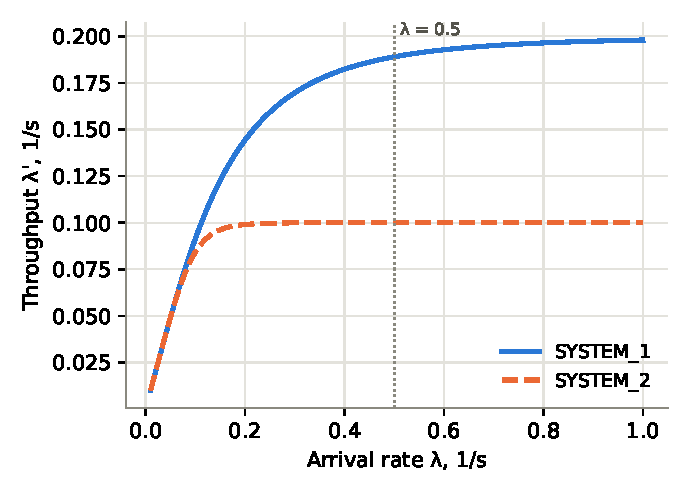
\includegraphics[width=\linewidth]{figures_en/thr.pdf}\caption{Throughput}\label{fig:thr}\end{subfigure}
\begin{subfigure}{0.49\textwidth}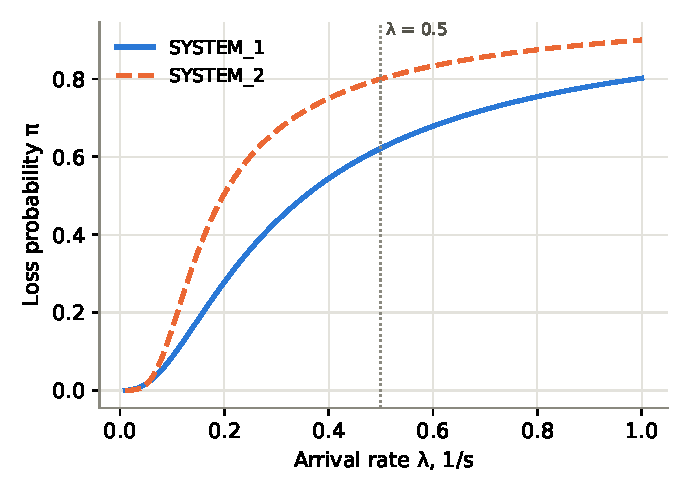
\includegraphics[width=\linewidth]{figures_en/loss.pdf}\caption{Loss probability}\end{subfigure}
\begin{subfigure}{0.49\textwidth}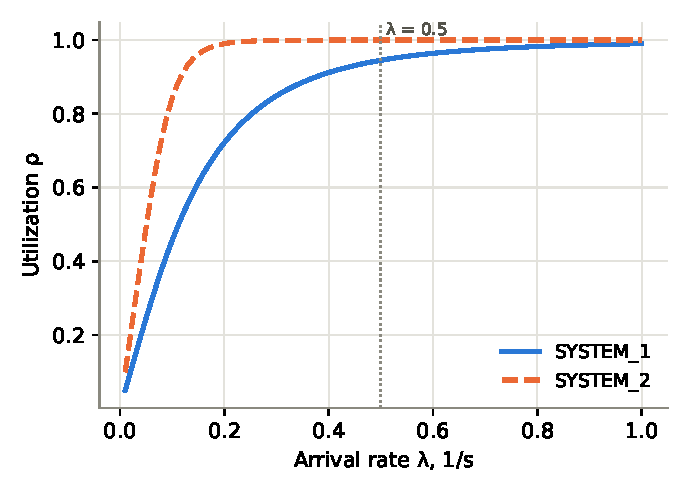
\includegraphics[width=\linewidth]{figures_en/rho.pdf}\caption{Utilization}\end{subfigure}
\begin{subfigure}{0.49\textwidth}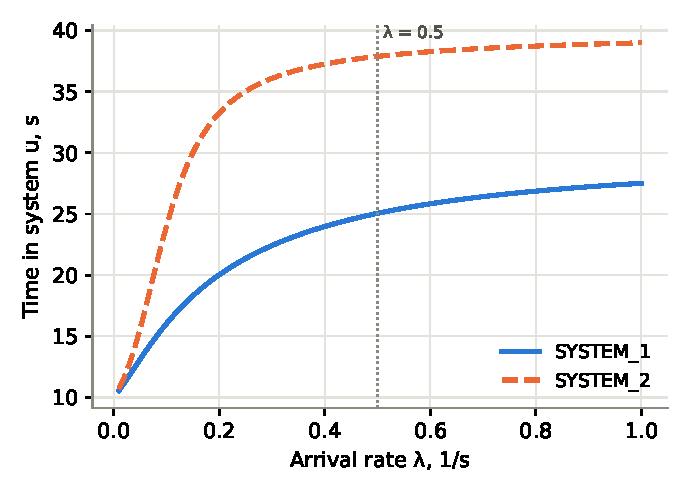
\includegraphics[width=\linewidth]{figures_en/u.pdf}\caption{Time in system}\end{subfigure}
\begin{subfigure}{0.49\textwidth}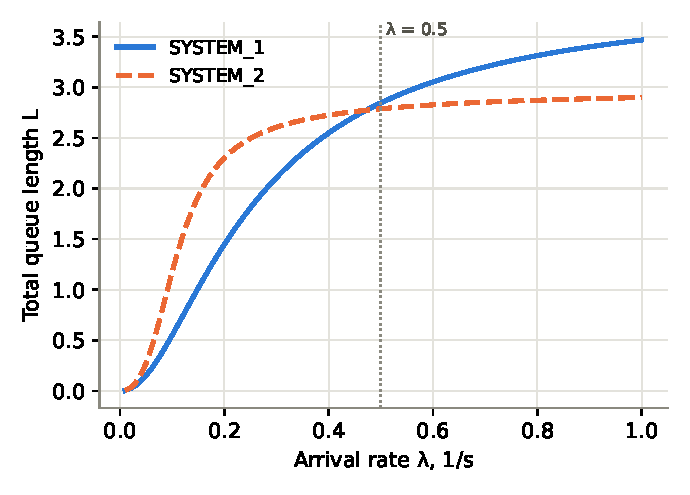
\includegraphics[width=\linewidth]{figures_en/queue.pdf}\caption{Total queue length}\end{subfigure}
\begin{subfigure}{0.49\textwidth}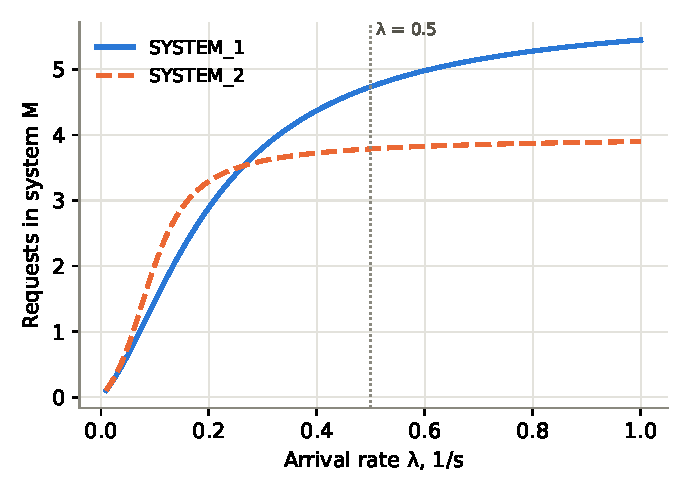
\includegraphics[width=\linewidth]{figures_en/m.pdf}\caption{Requests in system}\label{fig:m}\end{subfigure}
\caption{System characteristics versus $\lambda$ (dotted line: the given value $\lambda = 0.5$)}
\end{figure}

The plots show:
\begin{itemize}
\item At low arrival rates ($\lambda \lesssim 0.05$ 1/s) the throughputs of the two systems practically
coincide and equal $\lambda$, because losses are small. As $\lambda$ grows, SYSTEM\_2 quickly saturates at
$1/b = 0.1$ 1/s, while SYSTEM\_1 keeps growing towards its limit of $0.2$ 1/s. Hence
$\Lambda'_1 \ge \Lambda'_2$ for every $\lambda$.
\item SYSTEM\_2 has lower losses only for $\lambda < 0.054$ 1/s (there one shared buffer of 3 places is
more efficient than two separate buffers of 2); at higher rates SYSTEM\_1 loses less.
\item The server of SYSTEM\_2 is always more utilized: a single server takes the whole flow, whereas in
SYSTEM\_1 the flow is split between two servers.
\item Time in system is shorter in SYSTEM\_1 for every $\lambda$, and the gap widens with load.
\item The total queue length and the number of requests in SYSTEM\_1 exceed those of SYSTEM\_2 for
$\lambda > 0.47$ and $\lambda > 0.26$ 1/s respectively, because SYSTEM\_1 has a larger total capacity
(2 servers + 4 places versus 1 server + 3 places). At the given $\lambda=0.5$ this shows only as a
slightly larger $L$.
\end{itemize}

\subsection{Effect of request routing in SYSTEM\_1}
\begin{figure}[H]
\centering
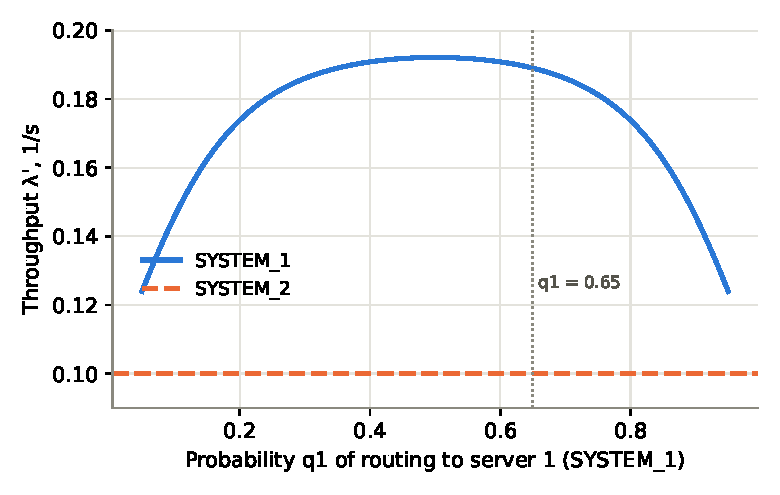
\includegraphics[width=0.6\textwidth]{figures_en/routing.pdf}
\caption{Throughput of SYSTEM\_1 versus routing probability $q_1$}
\end{figure}
SYSTEM\_1 reaches its maximum throughput with an even split ($q_1 = 0.5$): \SoneSymThr\ 1/s. At the given
$q_1=0.65$ it is only $\approx 1.6\,\%$ lower, and for every $q_1 \in [0.05,\,0.95]$ SYSTEM\_1 stays
ahead of SYSTEM\_2.

% ======================= 9 =======================
\section{Choice of the best system}
The efficiency criterion is \textbf{maximum system throughput} (the rate of the flow of served
requests, $\Lambda'$):
\[
\Lambda'_1 = \SoneThr \ \text{1/s} \;>\; \Lambda'_2 = \StwoThr \ \text{1/s}.
\]
\textbf{The best option is SYSTEM\_1} (two exponential servers with separate buffers of capacity 2/2):
its throughput is \Ratio\ times higher. SYSTEM\_1 is also better in loss probability and time in system;
SYSTEM\_2 wins only on single-server utilization and, marginally, on total queue length, neither of which
is the given criterion. The conclusion holds for any arrival rate: at small $\lambda$ the throughputs
coincide, and as $\lambda$ grows the advantage of SYSTEM\_1 increases.

% ======================= 10 =======================
\section{Conclusion}
Markov models were built for two queueing systems: a two-server system with separate buffers
(16 states) and a single-server system with 3rd-order Erlang service (13 states, method of phases).
For each system the labelled transition graph and the transition rate matrix were constructed, the
stationary probabilities were computed, and the full set of characteristics was derived from the state
probabilities; correctness was confirmed with the fundamental relations (Little's law and others).
By the maximum-throughput criterion, SYSTEM\_1 was chosen.

\appendix
\section*{Appendix A. Computation program (Python)}
\addcontentsline{toc}{section}{Appendix A. Computation program (Python)}
\lstinputlisting{code/model.py}

\end{document}
